\chapter[Partial internal non-life model \PODRA]{A partial internal model for a non-life insurance company: \PODRA}
\label{chap:podra}

The \PODRA{} Model\footnote{\PO{} Dynamic Reinsurance Analysis\cite{09:MunichRePodra}}
serves two purposes.  First, it is a fairly powerful non-life, primary insurance risk
model which can be used as a partial internal Solvency~II model.  Second, it can be used
as a starting point for developing custom models -- a topic which is taken up in more
advanced sections.  The \PODRA{} model is a typical representative of a dynamically
extendable model (see the classification of models in~\ref{ref:TODO}\todo{REF TO DO}{}).  We will use it
here for two reasons.  Firstly, because we can build a custom model with a reasonable,
pre-defined structure laid out by an expert, without any programming.  And secondly,
because it is a fully published model -- \ie, one can reproduce each of the steps below
after downloading the release -- making the first section below an effective tutorial.

Its components are the gross portfolio (underwriting information and claims generators),
the company structure and the reinsurance covers. Its output provides a good basis to
analyize capital at risk, premium, provisions and claims on different levels. Possible
uses are risk analyses, portfolio optimization and reinsurance structuring.

Please refer to a workshop held in September 2010 in St.Gallen for illustrative examples on  \href{http://pillarone.org/collaboration/events/saa-st.-gallen-2010/presentations/2-dynamic-analysis-of-an-insurance-portfolio}{pillarone.org}

\note{The \PODRA{} model is a data-driven model which can be easily extended by simply adding
input data for new claims generators, underwriting segments, etc. The price for this
flexibility is performance. If this flexibility is not needed, then there are ways to
build models with the same business logic which have about half the runtime of an
equivalent dynamic model.}

\section{Step by step}
\label{sec:podra-step}

The first step is to open the application and select the \PODRA{} model. Within the \PODRA{} 
model, we wish to start from scratch. Hence we use the context menu within \PODRA{} on
`Parametrisations' (right-mouse-click) to create a new default parametrisation. You will
find some more parametrisations within \PODRA/Parametrisations as examples. 
\todo{Screenshot}{example parameterizations}
Afterwards, name the newly created parametrisation and open it via the context menu
of the parametrisation itself.

In the right pane the (empty) model is shown.

The available segments that can be entered into the model are Underwriting, Claims Generators, Correlations, Lines of Business and Reinsurance Program.

\paragraph{Underwriting Information}
As a first step the underwriting information should be feeded into the model. Within the
Underwriting context menu there is a button add. Name the new Underwriting segment. Within
the segment, the data can be edited by doubleclick.
\begin{figure}
	\centering
		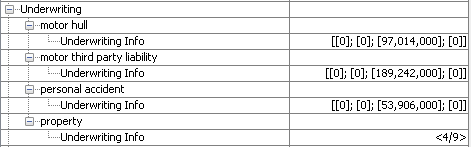
\includegraphics[scale=0.75]{images/podra-uwinfo.png}
	\caption{\PODRA{} underwriting information example}
	\label{fig:podra-uwinfo}
\end{figure}

The underwriting information contains: maximum sum insured, average sum insured, premium
and number of policies. It is possible to edit serveral risk bands (they will be used for
surplus share treaty reinsurance). Add as many Underwriting segments as you like.

Underwriting information is optional to some extent and can be either attached to a claims generator (see below) where it can be used for skaling of distributions or as exposure information for surplus reinsurance contracts; or it can be attached to a Line of Business \todo{where it is used to}{please explain}.

\paragraph{Claims Generators}
The next step is the editing of Claims Generators. Context menu \menu{add} creates a new claims
generator. Compared to the underwriting information a claims generator is more complex. It contains the claims model, the
exposure information association, and the underlying underwiting information.

For the claims generator the type of the claims generator can be selected:
\menu{Attritional}, \menu{Frequency Severity} and many more.
Depending on the selection there are different ways to define the claims generator appropriately.
The model starts with drawing a claim from the selected claims generator. If a surplus
share treaty will be contained in the reinsurance program, the second step is the allocation of an exposure (sum insured,
pml, eml) to the drawn loss. Therefore the option to selecting the exposure information
allocation can be used.

The combo box \todo{`claims generator is based on'}{check name} is used to scale the random distributions by
underwriting information from the underwriting segments. If no underwriting is provided or applicable, a given fixed value \term{absolute} van be selected.
\begin{figure}
	\centering
		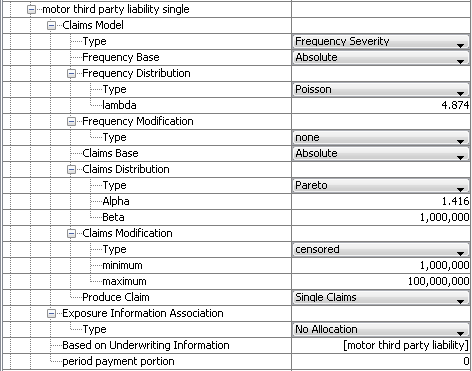
\includegraphics[scale=0.75]{images/podra-claimsgen.png}
	\caption{\PODRA{} claims generator example}
	\label{fig:podra-claimsgen}
\end{figure}
% ToDo: Period payment portion to be commented.

\paragraph{Correlations}
Claims generators may interact, or, in other words, correlate. Correlations can be introduced by adding a
Correlations Matrix using the Context Menu Add of \term{dependencies} on the right pane.

\paragraph{Reserve generators}
The reserve generators can be introduced like claims generators. The reserve generators
component allows for adding reserve generators for a certain segmentation. It contains the
reserve development (paid plus reserved) distribution possibly with modifiers.
Additionally the recent year payment portion can be specified to allow for very simple
reserve development modelling. Furthermore the initial reserves can be specified directly in
this component.
Within a multi period model the outgoing reserves of claims generators can be linked to
the reserve component, resulting in increasing the reserve volume of future periods by the amount of the outgoing reserve of the preceding period. 

\begin{figure}
	\centering
		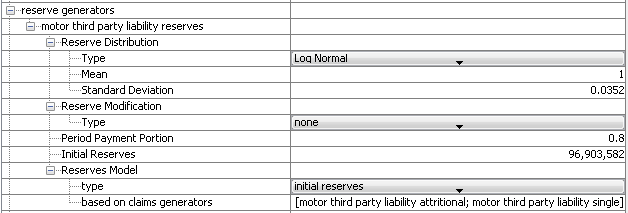
\includegraphics[scale=0.75]{images/podra-reservesgen.png}
	\caption{\PODRA{} reserve generator example}
	\label{fig:podra-reservegen}
\end{figure}

\paragraph{Lines of Business}
Now the risks are defined and may be combined or allocated on business segments. These are
defined in the Line of Business area. Here again, it is possible to add another Line of
Business. The next step is to add different Claims generators (or shares of them) to the
dedicated Line of Business. Additionally, to each Line of Business the Underwriting
Information is attached, so we can select this additionally.

\paragraph{Reinsurance Program}
Individual Reinsurance covers can be added to the Reinsurance Program section. The
reinsurance cover consists of a contract (including the type), the inuring priority (see further below), the
covered lines of business, as well as the covered claims generators. The covered lines of
business and the convered claims generators are sent to the reinsurance contract to be
covered.

\begin{figure}
	\centering
		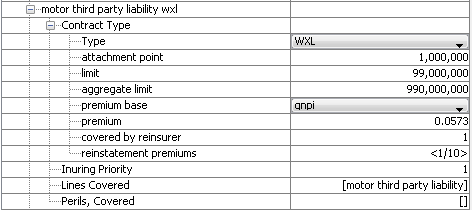
\includegraphics[scale=0.75]{images/podra-reinsurance.png}
	\caption{\PODRA{} reinsurance contract example}
	\label{fig:podra-ri-contract}
\end{figure}

The inuring priority provides the information when a specific contract is used and from
which level \eg the GNPI is taken. For the reinsurance program itself the type has to be
specified. Depending on the type there are several options for the necessary parameters.

\paragraph{Result configuration}
Usually, not all possible result variables are generated and stored during a
simulation run. This is for performance and disk space reasons. Within the \PODRA{} model several result configurations can be defined. By opening a result descriptor
in the right pane a tree view with the available output variables is shown. On each output
variable a collection type can be selected. To make a result variable available in the
result set, it should be collected as aggregated or drill down\todo{ref to new section}{please include ref}. This output variables will be found in
the Results after a simulation has been done.

\todo{Screenshot}{Result Configuration}

\paragraph{Evaluation / Simulation} 
On Parameters and Result Descriptors within the left tree view it is possible
to start simulations using the context menu. The Parameter set and the Result Descriptor to be used have to be selected in the Simulation window on the right pane.
The simulation run can be started after adding the number of simulatons and optionally
the random generator seed. The Results of the \PODRA{} model will contain your result set thereafter.

Open the result set to see which variables have been generated. On the result
variables different risk measures (exactly different functionals) can be displayed
by pressing the appropriate buttons. The diverse options for evaluations include
expected value, standard deviation, value at risk and tail value at risk for a given
level of \todo{security}{confirm wording}. The full set -- or any branch of the tree -- can be copied to the clipboard by selecting the top element of the branch or tree respectively and pressing ctrl-c.

\todo{Screenshot}{Evaluation - simulation}

Given the model has been evaluated twice with different parameters the results can be
compared using the compare feature selectable in the treeview. Deviations in all result
variables can be shown in absolute and relative form. Sensitivity tests of paramerters
can be done easily using this feature.

\todo{Screenshot}{Compare}